\documentclass[letterpaper, 12pt] {article}
\usepackage[table,xcdraw, caption]{xcolor}
\usepackage{amsmath}
\usepackage{todonotes}
\usepackage{graphicx}
\usepackage[normalem]{ulem}


% The follwing changes the margin text size
\let\oldmarginpar\marginpar
\renewcommand\marginpar[1]{\-\oldmarginpar[\raggedleft\footnotesize #1]%
	{\raggedright\footnotesize #1}}
%%%%%%%%%%%%%%%%%

\begin{document}

	
	\title{Algorithmic Trading}
	
	% Removes the date entry in article class
	\date{\vspace{-5ex}}
	\maketitle
	
	\begin{abstract}
	In the analysis of financial time series data, techniques like support and resistance are very popular amongst traders. This text presents an approach using which the  reader can quantitatively anticipate price movements in the near future, given some data. 
	\end{abstract}

	\section{\textbf{Basic Terminology}}
	
	Support and Resistance are used in technical analysis of stock prices. Techincal analysis involves observing the trend and patterns in financial data and trying to quantitatively predict the price movement. We briefly describe the terms "\textbf{Support}" and "\textbf{Resistance}" below-
	
	\paragraph{Support} A support level is a trendline where the price tends to find "support" as it falls. Traders believe that the price is more likely to bounce off this level rather than break through it. At this price level, demand is thought to be strong enough to prevent the price from declining any further. However, once the price breaches this level, traders redefine a new support, taking into account the recent lag data. Buyers purchase shares of a stock near the support level, as the price of the stock is expected not to decrease.
	
	\paragraph{Resistance} Resistance is, in some sense, a complement to the support. Resistance refers to the historicaly observed upper bound of the price of a stock, and  is expected to less likely be breached. At this price level, selling of a stock is thought to be strong enough to prevent the stock price from rising further. However, once the price has breached this level, the traders redefine a new resistance level taking into account the recent lag data. 
	
	\footnote{Should I add a representative figure for Support and Resistance???}
	
	
	\paragraph{} Both resistance and support are characterized by straight lines in the given time series data. Taken together, they give a quantitative forecast of a range of price movements.  

	\section{Approach}
	We describe an approach for a given data series with each price point located at a discretized fixed length from each other, say for example, like the represenative data series given below:-

	
	\begin{table}[h!]
		\centering
		\caption {Apple Data} \label{tab:} 
		
		\begin{tabular}{|c|c|}
			\hline
			\rowcolor[HTML]{C0C0C0} 
			{\color[HTML]{9A0000} { \textbf{Date}}} & {\color[HTML]{9A0000} {\textbf{Closing Price (in \$)}}} \\ \hline
			2017-08-23                                 & 157.597                                                     \\ \hline
			2017-08-24                                 & 156.897                                                     \\ \hline
			2017-08-25                                 & 157.478                                                     \\ \hline
			2017-08-28                                 & 159.064                                                     \\ \hline
			2017-08-29                                 & 160.483                                                     \\ \hline
			2017-08-30                                 & 160.916                                                     \\ \hline
		\end{tabular}
	\end{table}
	
	\paragraph{}
	It is seen that the Closing price is recorded at one day intervals. Now assume we are given data of length $n$ i.e, $n$ observations are recorded. The most intuitive thing to do is plot out the entire data series. (Refer Figure 1. on next page.)
	\begin{figure}[h!]
		\centering
		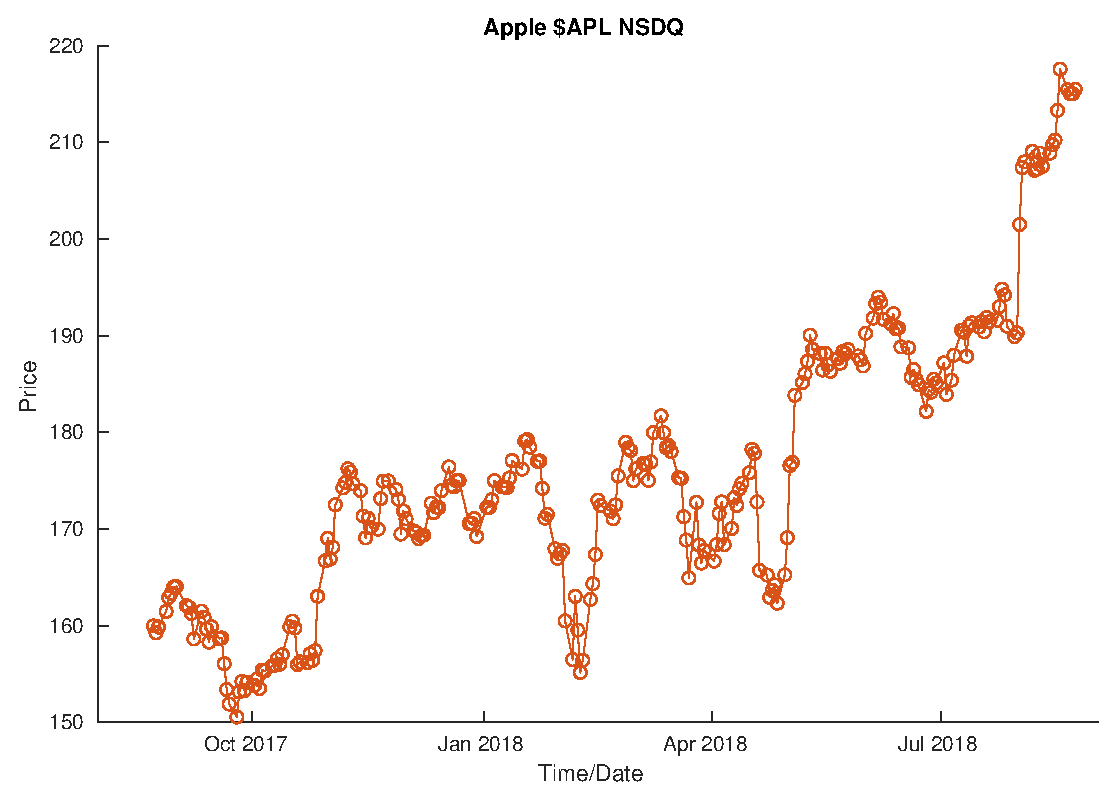
\includegraphics[scale = 0.45]{apple_c_plot_latex_raw}
		\caption{Apple Stock Price over FY 2017-2018}
		\label{Figure 1}
		
	\end{figure}
	
	\paragraph{}
	We then realize that in order to find the lines that correspond to \textit{Support} and \textit{Resistance} we \textbf{cannot} use the entire data series obtained by us, because doing so can give us an inaccurate representation of the trends \footnote{Should I add a figue here that shows why??}. It intuitively follows that we must choose a particular window of observations, \textbf{\textit{'l'}} called \textbf{lags} \footnote{\textit{the term lags will typically mean the number of observations that are considered while computing the trendlines.}}, the value of which will let us qualitatively plot the $Support$ and $Resistance$. Once we choose a particular value of \textit{'l'}, we can then proceed to find out the equation of lines that correspond to $Support$ and $Resistance$ trendlines. Once this is done, we can then determine the time interval till which the $Support$ and $Resistance$ line is obeyed. The motivation behind this approach is to plot an empirical distribution of \textit{time intervals} vs \textit{lags} within which the $Support$ and $Resistance$ trendlines are obeyed. \linebreak
	We rigorously state our goals, in the following paragraph.
	
	
	\section{Formalizing the Goals!}
	Suppose we are given a tuple $\{S_t = \$\ ,\ t = 0, 1,2, ..., n\}$ corresponding to a stock data series, where $S_t$ represents the price point of the said stock at corresponding $t$ \footnote{Note that $t$ can also represent the index of a list of $S_t$ if such a list is made.}. 
	\paragraph{}
	We denote the "present time" by $t$, (\textit{Note that this 't' is different from the above mentioned t, which implies the location of $S_t$ data point}). Now, given a value of $l$, where it denotes the units of lag, i.e, the number of observations before $t$, that are to be considered while estimating the trendlines for $Support$ and $Resistance$. It follows then that the term \textit{lagdata} corressponds to the tuple
	\begin{equation*}
	lagdata = \{S_{t-i}, t-i\}, \text{such that i} \; \epsilon \;[0, l]
	\end{equation*} 
	
	We have $|lagdata|$ a set of [$l+1$] points. We now restrict our attention to the $lagdata$ set and consider the collection of all the lines that pass through \textbf{\textit{any}} two points in the $lagdata$ set. It immediately is apparent that there are too many such lines possible. 
	\paragraph{}
	Our purpose is to choose a pair of trendlines such that-
	
	\begin{description}
		\item[$\bullet$] The trendlines contain all the points $\; \epsilon\; lagdata $ in their spread
		\footnote{see figure 2.}.
		\item[$\bullet$] The spread of the trendlines chosen is the \textbf{\textit{least}}
	\end{description}
	
	\begin{figure}[h!]
		\centering
		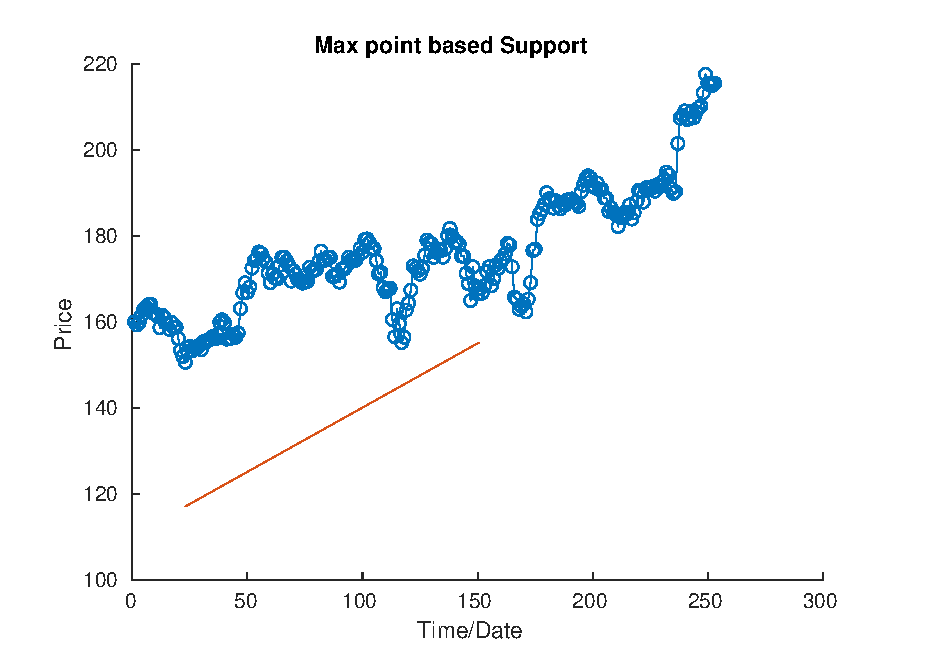
\includegraphics[scale = 0.45]{max_supp}
		\caption{One of the many possible "\textit{Support}" lines}
		\label{Figure 2}
	\end{figure}
	
	\paragraph{}
	In order to satify the desired conditions, we bring in a minimization problem. The benefit of doing so is the ability to choose a 'unique' line. For example, if we consider the data points that make up the $lagdata$ set, the plot effected by our selection can be considered analogous to a piece of metal wire having the same 2-D geometry as $lagdata$. Computing a trendline that is closest to the data is possible only if we have some global parameter with which we compare all possible 'best' fits. One global parameter readily follows from the visualization just made. We simply minimize the distance of the center of gravity of the dataset (visualized as a metal piece), to the trendline that contain the dataset within their spread \footnote{see figure 3.}.This minimizaion can be acheived by "moving" the computed trendlines wrt the global parameter.   
	
	\begin{figure}[h!]
		\centering
		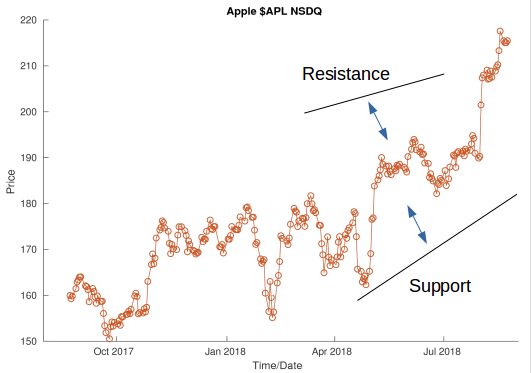
\includegraphics[width=0.8\textwidth]{cogs_minimize}
		\caption{Moving the "\textit{Support}" and \textit{"Resistance"} lines}
		\label{Figure 3}
	\end{figure}
	
	We explicitly outline the details below- \pagebreak
	
	\subparagraph{Computing the Trendlines}
	Assume that the center of gravity is located at $g = (g_1, g_2)$ in the x-y plane. It immediately follows that the $x$ component of the tuple $(g_1, g_2)$ is located at $x = [t - \frac{l}{2}]$. This is because the points are given equal weights, ie the Center of Gravity will lie at the center of the x-projection of the line. The $y$ component of the tuple $(g_1, g_2)$ would then be located at $y = [\frac{1}{l+1}\sum_{s=0}^{l} X_s ]$\footnote{Should I explain this???}. i.e -
	
	\begin{equation*}
	(g_1, g_2) = (t - \frac{l}{2}, \frac{1}{l+1}\sum_{s=0}^{l} X_s )
	\end{equation*}
	
	We now choose two points $(s_1, X_(s1))$ and $(s_2, X_(s2))$ in the set $lagdata$. Given these two points, the equation of line that passes through them is given by\footnote{give any explanation??} 
	$$L = X_{s_1} + \frac{X_{s_2} - X_{s_2}}{s_2 - s_1}(s - s_1)$$ 
	The tuple $(s, L(s))$ is the locus of the desired line $L$. 
	
	\paragraph{}
	Now that we have the locus of the line $L$, we move the line towards or away from the center of gravity. Let $J(s_1, s_2)$ be the perpendicular distance between the point $(g_1, g_2)$ and the line. Then, \footnote{\label{note9}Again!!!... Should we explain this??} we have-
	
	\begin{equation*}
	J(s_1, s_2) = \frac{|X_{s_1} - X_{s_2}|g_1- (s_2-s_1)g_2 +(X_{s_1}s_2 - X_{s_2}s_1)}{\sqrt{(X_{s_1} - X_{s_2})^2 + (s_2 - s_1)^2}}
	\end{equation*}
	
	We obtain the equation for $support$ by solving the minimization problem described below-
	
	\begin{equation*}
	\text{min}\;_{{t-l}\leq {s_1} < {s_2} \leq t} \; J(s_1, s_2) \; \text{subject to} \{X_k \geq L(k; s_1, s_2) \forall \; 0 \leq k \leq l\}. 
	\end{equation*}
	
	Let $(s_1', s_2')$ be the minimizer for the above statement, we then can show that the equation of support is given by:
	
	\begin{equation*}
		L(s) = X_{s_1'} + \frac{X_{s_2'}-X_{s_1'}}{s_2' - s_1'} (s-s_1')
	\end{equation*}
	
	The equation of resistance can then be obtained by a similar approach \marginpar{refer to footnote 9}.
	\linebreak
	
	\textbf{Empirical Distribution of $\delta^+(l)$ and $\delta^-(l)$}: blah balah basjkahdkjhka
	 	
	

\end{document}